Второй вариант архитектуры компонента Remap, содержащий память FIFO, представлен на рисунке \ref{fig:remap_fifo}.\par
\begin{figure}[ht]
    \centering
    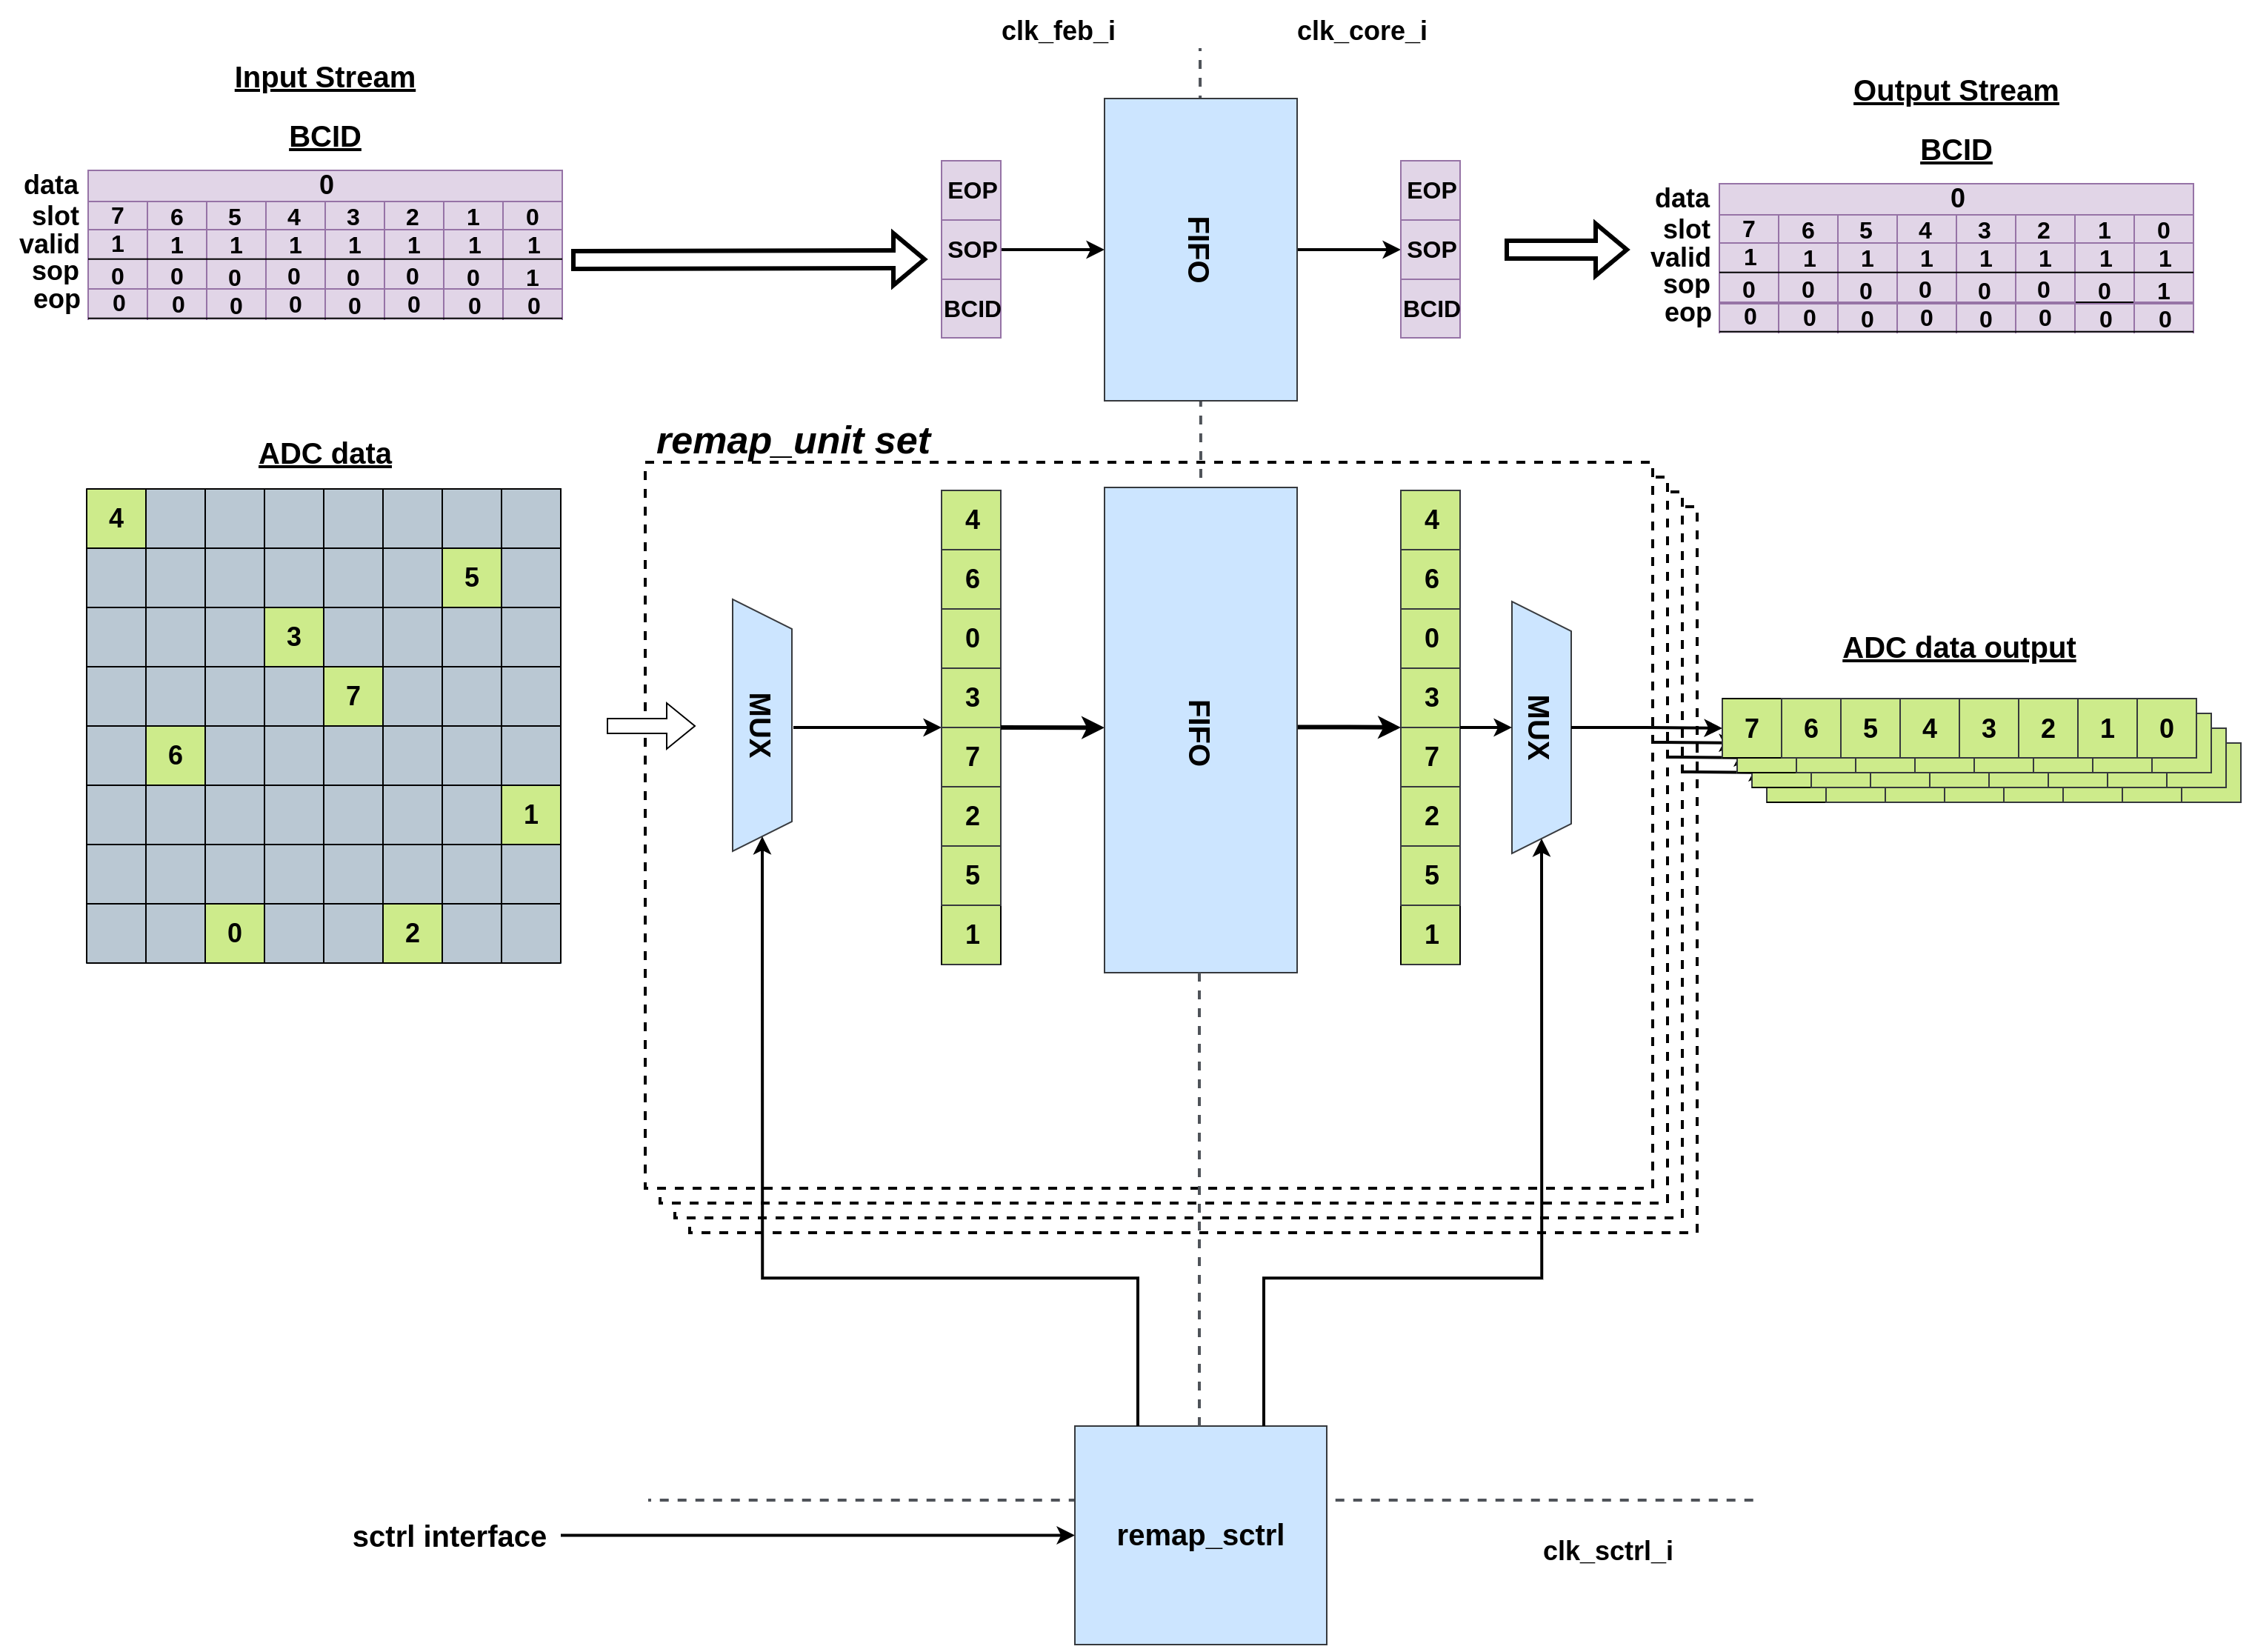
\includegraphics[width=\linewidth]{remap_fifo.png}
    \caption{Схема архитектуры модуля Remap, основанной на FIFO ПЕРЕВЕСТИ}
    \label{fig:remap_fifo}
\end{figure}\par
В рамках данного подхода в качестве буфера для мультиплексированных данных является память FIFO (First In First Out). Такая структура состоит из двухпортовой памяти, двух счётчиков адреса и двух автоматов для чтения и записи данных и является одним из ключевых элементов цифровой схемотехники. Одно из самых распространённых применений такой памяти, помимо буферизации информации -- это реализация перехода данных между тактовыми доменами. Поскольку такая память используется невероятно часто в проектировании логических схем, то существует множество готовых вариантов их реализации, в том числе и от разработчиков самих микросхем ПЛИС и соответствующего программного обеспечения для автоматического проектирования, в том числе и от Intel. В случае использования такого готового блока FIFO не требуется ручное написание временных ограничений, что избавляет от потенциальных проблем на этапе синтеза цифровой схемы всего проекта.\par
Однако, одна из основных особенностей FIFO -- это сохранение порядка записываемых данных, что не позволяет реализовать последний этап работы модуля Remap. Для решения данной задачи используется подход, при котором данные с мультиплексора поступают не напрямую на вход FIFO, а записываются в один большой регистр, достаточного размера для одновременного хранения всех мультиплексированных данных в рамках текущего столкновения пучков. Для наиболее оптимального использования логических ресурсов этот регистр является сдвиговым, то есть каждый такт новое значение поступает в начало, после чего оно смещается дальше. Только после полного заполнения этого регистра актуальными величинами, данные одним большим словом записывается в FIFO. Считывающая логика, после обнаружения данных на выходе FIFO, имеет доступ сразу ко всем значениям и может извлекать их последовательно в необходимом порядке.\par
В целях минимизации латентности необходимо, чтобы поступающие в FIFO данные сразу же были доступны для чтения, то есть требуется не допускать его заполнения. Поскольку запись и извлечение идёт с одной и той же скоростью, важно важно сделать так, чтобы считывающая система начала работу как минимум не позднее записывающей. Это достигается правильным управлением сигналами сброса: после старта сигнального процессора LASP сначала должен сняться сброс, синхронный с тактовым доменом $f_{core}$, а уже затем $f_{feb}$.\par
В случае возникновения каких-то ошибок может возникнуть ситуация, когда FIFO заполнится и записывающая сторона не сможет сохранить новые данные. Для обработки такого случая перед записью каждой новой порции информации осуществляется проверка состояния буфера. Если оказывается, что блок FIFO заполнен, то текущие данные отбрасываются и инкрементируется счётчик ошибок, который доступен по чтению через интерфейс медленного контроля. Такой счётчик может быть жизненно необходим для отладки на этапе аппаратного запуска системы на целевой платформе, потому что это один из самых доступных способов узнать состояние модулей во время их непосредственной работы.\par
